\documentclass[12pt, oneside]{article}
\usepackage[T1]{fontenc}
\usepackage[spanish, es-tabla, es-lcroman]{babel}
\usepackage[utf8]{inputenc}
\usepackage[document]{ragged2e}
\usepackage{tcolorbox}
\tcbuselibrary{theorems}
\usepackage{cancel}
\usepackage{amssymb}
\usepackage{amsmath}
\usepackage{mathrsfs}
\usepackage{wrapfig}
\usepackage{fancyhdr}
\usepackage{colortbl}
\usepackage{longtable}
\usepackage{diagbox}
\usepackage{graphicx}
\usepackage{subcaption}
\usepackage{xcolor}
\usepackage{tikz}
\usetikzlibrary{positioning}
\usepackage{multicol}
\usepackage{multirow}
\usepackage{lastpage}
\usepackage{pdfpages}
\usepackage{listings}
\usepackage{blindtext}
\spanishdecimal{.}
\usepackage[explicit]{titlesec}
\usepackage[colorlinks=true, linkcolor=black, citecolor=black, urlcolor=blue]{hyperref}
\usepackage[a4paper, total={16cm, 24cm}]{geometry}
\pagestyle{fancy}
\lhead{Muñoz Nuñez Ian Emmanuel}
\rhead{Proyecto 9}
\lfoot{Mtra. María Patricia Ventura Nuñez}
\rfoot{CUCEI}
\renewcommand{\headrulewidth}{1pt}
\renewcommand{\footrulewidth}{1pt}

\setlength{\headheight}{14.49998pt}
\definecolor{rojo}{RGB}{255, 0, 0}
\definecolor{azul}{RGB}{0, 0, 255}

\definecolor{basicPLD}{RGB}{160, 160, 160}
\definecolor{fondoPLD}{RGB}{40, 40, 40}
\definecolor{commentPLD}{RGB}{0, 240, 170}
\definecolor{keywordsPLD}{RGB}{0, 170, 240}

\lstdefinestyle{SPPSR}{
basicstyle=\ttfamily\small\color{basicPLD},
backgroundcolor=\color{fondoPLD},
commentstyle=\color{commentPLD},
numbers=left,
numberstyle=\ttfamily\small\color{black},
numbersep=5pt,
breaklines=true,
keepspaces=true,
showspaces=false,
showstringspaces=false,
showtabs=false,
xleftmargin=10pt,
emph={PIN, \$DEFINE, FIELD, SEQUENCE, PRESENT, IF, NEXT},
emphstyle=\color{keywordsPLD},
rulesepcolor=\color{magenta},
frame=shadowbox
}
\lstset{style=SPPSR}

\begin{document}

\begin{titlepage}
    \pagenumbering{roman}
    \centering
    {\bfseries\LARGE Universidad de Guadalajara \par}
    \vfill
    {
        \includegraphics[width=0.3\linewidth]{UdG.png}
        \includegraphics[width=0.3\linewidth]{qci.png}
        \par
    }
    \vfill
    {\bfseries\LARGE Seminario de problemas de programación de sistemas reconfigurables \par}
    \vfill
    {\ttfamily\LARGE Contador del 0 al 9 con \emph{BCD (8, 4, -2, -1)} \par}
    \vfill
    {\bfseries\LARGE Nombre: \par}
    \vfill
    {\bfseries\LARGE Muñoz Nuñez Ian Emmanuel \par}
    \vfill
    {\bfseries\LARGE Sección: D01 \par}
    \vfill
    {\bfseries\LARGE Código: 216464457 \par}
    \vfill
    {\bfseries\LARGE Maestra: \par}
    \vfill
    {\bfseries\LARGE María Patricia Ventura Nuñez \par}
    \vfill
    {\bfseries\LARGE Ingeniería Robótica \par}
\end{titlepage}

\pagenumbering{arabic}

\newpage
\section{Objetivo}
{\sffamily\large
    \hspace{0.5cm} Solucionar problemas de diseño utilizando las herramientas aprendidas
    en programación de sistemas reconfigurables.

    \hspace{0.5cm} Simular circuitos digitales en programas de diseño como
    \emph{Proteus\textregistered} e implementarlos físicamente.

    \hspace{0.5cm} Diseño e implementación de un contador asíncrono del 0 al 9 utilizando
    \emph{F-F JK} con código \emph{BCD (8, 4, -2, -1,)}.

}

\section{Material}
{\sffamily\large
    \renewcommand{\labelitemi}{$\bullet$}
    \begin{itemize}
        \item Protoboard.
        \item Fuente VCC (5V).
        \item Resistencias de $220\Omega$ y $2k\Omega$.
        \item Dip-switch de 4 bits.
        \item 4 leds.
        \item 4 \emph{F-F JK 4027}.
        \item \emph{GAL22v10D}.
    \end{itemize}
}

\newpage
\section{Marco teórico}
\subsection{Código BCD (8, 4, -2, -1)}
{\sffamily\large
    \begin{table}[h!]
        \centering
        \sffamily
        \scalebox{1.5}{
        \begin{tabular}{|c||c|c|c|c|}
            \hline
            & 8 & 4 & -2 & -1 \\
            \hline
            0 & 0 & 0 & 0 & 0 \\
            \hline
            1 & 0 & 1 & 1 & 1 \\
            \hline
            2 & 0 & 1 & 1 & 0 \\
            \hline
            3 & 0 & 1 & 0 & 1 \\
            \hline
            4 & 0 & 1 & 0 & 0 \\
            \hline
            5 & 1 & 0 & 1 & 1 \\
            \hline
            6 & 1 & 0 & 1 & 0 \\
            \hline
            7 & 1 & 0 & 0 & 1 \\
            \hline
            8 & 1 & 0 & 0 & 0 \\
            \hline
            9 & 1 & 1 & 1 & 1 \\
            \hline
        \end{tabular}
        }
        \caption{\sffamily Tabla del código BCD 8 4 -2 -1}
        \label{tab:bcd}
    \end{table}
}

\subsection{Tabla de verdad}
{\sffamily\large
    \begin{table}[h!]
        \centering
        \sffamily
        \scalebox{0.9}{
        \begin{tabular}{|c||c|c|c|c||c|c|c|c||c|c|c|c||c|c||c|c|}
            \hline
            & QB & * & * & * & \multicolumn{4}{c||}{$Q^t$} & \multicolumn{4}{c||}{$Q^{t+1}$} & \multicolumn{2}{c||}{B} & \multicolumn{2}{c|}{C} \\
            \hline
            & QA & QB & QC & QD & QA & QB & QC & QD & QA & QB & QC & QD & JB & KB & JC & KC \\
            \hline
            0 &  0 & 0 & 0 & 0 &  0 & 0 & 0 & 0 &  0 & 1 & 1 & 1 &  1 & X & 1 & X \\
            \hline
            1 &  0 & 1 & 1 & 1 &  0 & 0 & 0 & 1 &  X & X & X & X &  X & X & X & X \\
            \hline
            2 &  0 & 1 & 1 & 0 &  0 & 0 & 1 & 0 &  X & X & X & X &  X & X & X & X \\
            \hline
            3 &  0 & 1 & 0 & 1 &  0 & 0 & 1 & 1 &  X & X & X & X &  X & X & X & X \\
            \hline
            4 &  0 & 1 & 0 & 0 &  0 & 1 & 0 & 0 &  1 & 0 & 1 & 1 &  X & 1 & 1 & X \\
            \hline
            5 &  1 & 0 & 1 & 1 &  0 & 1 & 0 & 1 &  0 & 1 & 0 & 0 &  X & 0 & 0 & X \\
            \hline
            6 &  1 & 0 & 1 & 0 &  0 & 1 & 1 & 0 &  0 & 1 & 0 & 1 &  X & 0 & X & 1 \\
            \hline
            7 &  1 & 0 & 0 & 1 &  0 & 1 & 1 & 1 &  0 & 1 & 1 & 0 &  X & 0 & X & 0 \\
            \hline
            8 &  1 & 0 & 0 & 0 &  1 & 0 & 0 & 0 &  1 & 1 & 1 & 1 &  1 & X & 1 & X \\
            \hline
            9 &  1 & 1 & 1 & 1 &  1 & 0 & 0 & 1 &  1 & 0 & 0 & 0 &  0 & X & 0 & X \\
            \hline
            10 &  & & & &  1 & 0 & 1 & 0 &  1 & 0 & 0 & 1 &  0 & X & X & 1 \\
            \hline
            11 &  & & & &  1 & 0 & 1 & 1 &  1 & 0 & 1 & 0 &  0 & X & X & 0 \\
            \hline
            12 &  & & & &  1 & 1 & 0 & 0 &  X & X & X & X &  X & X & X & X \\
            \hline
            13 &  & & & &  1 & 1 & 0 & 1 &  X & X & X & X &  X & X & X & X \\
            \hline
            14 &  & & & &  1 & 1 & 1 & 0 &  X & X & X & X &  X & X & X & X \\
            \hline
            15 &  & & & &  1 & 1 & 1 & 1 &  0 & 0 & 0 & 0 &  X & 1 & X & 1 \\
            \hline
        \end{tabular}
        }
        \caption{\sffamily Tabla de verdad para el circuito}
        \label{tab:tablaVerdad}
    \end{table}
}

\subsection{Ecuaciones logicas}
{\sffamily\large
    \begin{figure}[h!]
        \centering
        \includegraphics[width=0.5\linewidth]{figs/jb0.png}
        \caption{\sffamily Diagrama de \emph{Karnaugh} para obtener \emph{JB}}
        \label{fig:karJB}
    \end{figure}

    \begin{equation*}
        JB =
        \mathbf{
            \textcolor{rojo}{\overline{QC}\, \overline{QD}}
        }
    \end{equation*}

    \begin{figure}[h!]
        \centering
        \includegraphics[width=0.5\linewidth]{figs/kb0.png}
        \caption{\sffamily Diagrama de \emph{Karnaugh} para obtener \emph{KB}}
        \label{fig:karKB}
    \end{figure}

    \begin{equation*}
        KB =
        \mathbf{
            \textcolor{rojo}{\overline{QC}\, \overline{QD}}
            + \textcolor{azul}{QA}
        }
    \end{equation*}

}

\newpage
{\sffamily\large
    \begin{figure}[h!]
        \centering
        \includegraphics[width=0.5\linewidth]{figs/jc0.png}
        \caption{\sffamily Diagrama de \emph{Karnaugh} para obtener \emph{JC}}
        \label{fig:karJC}
    \end{figure}

    \begin{equation*}
        JC =
        \mathbf{
            \textcolor{rojo}{\overline{QD}}
        }
    \end{equation*}

    \begin{figure}[h!]
        \centering
        \includegraphics[width=0.5\linewidth]{figs/kc0.png}
        \caption{\sffamily Diagrama de \emph{Karnaugh} para obtener \emph{KC}}
        \label{fig:karKC}
    \end{figure}

    \begin{equation*}
        KC =
        \mathbf{
            \textcolor{rojo}{QA\, QB} + \textcolor{azul}{\overline{QD}}
        }
    \end{equation*}
}

\newpage
\subsection{Código}
\begin{lstlisting}[
    language=c,
    caption={\sffamily Código desarrollado en \emph{WinCupl}}]
Name     proy9 ;
PartNo   00 ;
Date     11/03/2022 ;
Revision 01 ;
Designer ian ;
Company  ianemn ;
Assembly None ;
Location  ;
Device   g22v10 ;

/* ENTRADAS */
PIN 2=QA;
PIN 3=QB;
PIN 4=QC;
PIN 5=QD;

/* SALIDAS */
PIN 23=JB;
PIN 22=KB;
PIN 21=JC;
PIN 20=KC;

JB = !QC & !QD;
KB = (!QC & !QD) # QA;
JC = !QD;
KC = (QA & QB) # !QD;
\end{lstlisting}

\newpage
\section{Procedimiento}
{\sffamily\large
    \hspace{0.5cm} Primero se hizo la representación de los numeros en código
    \emph{BCD (8, 4, -2, -1)}. Después se observó la forma de controlar los estados
    de forma asíncrona y se hizo la tabla de verdad para el circuito.

    \hspace{0.5cm} Con la tabla de verdad se obtuvieron las ecuaciones lógicas para
    realizar las conexiones del circuito y para programar la \emph{GALL22v10}.

    \hspace{0.5cm} Los materiales utilizados son: 1 dip-switch de 4 bits, 4 resistencias
    de $220\Omega$ y una de $2k\Omega$, 4 leds, 2 \emph{Flip-Flop's 4027}, una
    \emph{GAL22v10} y un generador de pulsos de reloj.

}

\section{Circuito a implementar}
\subsection{Simulación}
{\sffamily\large
    \hspace{0.5cm} En la siguiente página se muestra el diseño del circuito en simulación.

    \newpage
    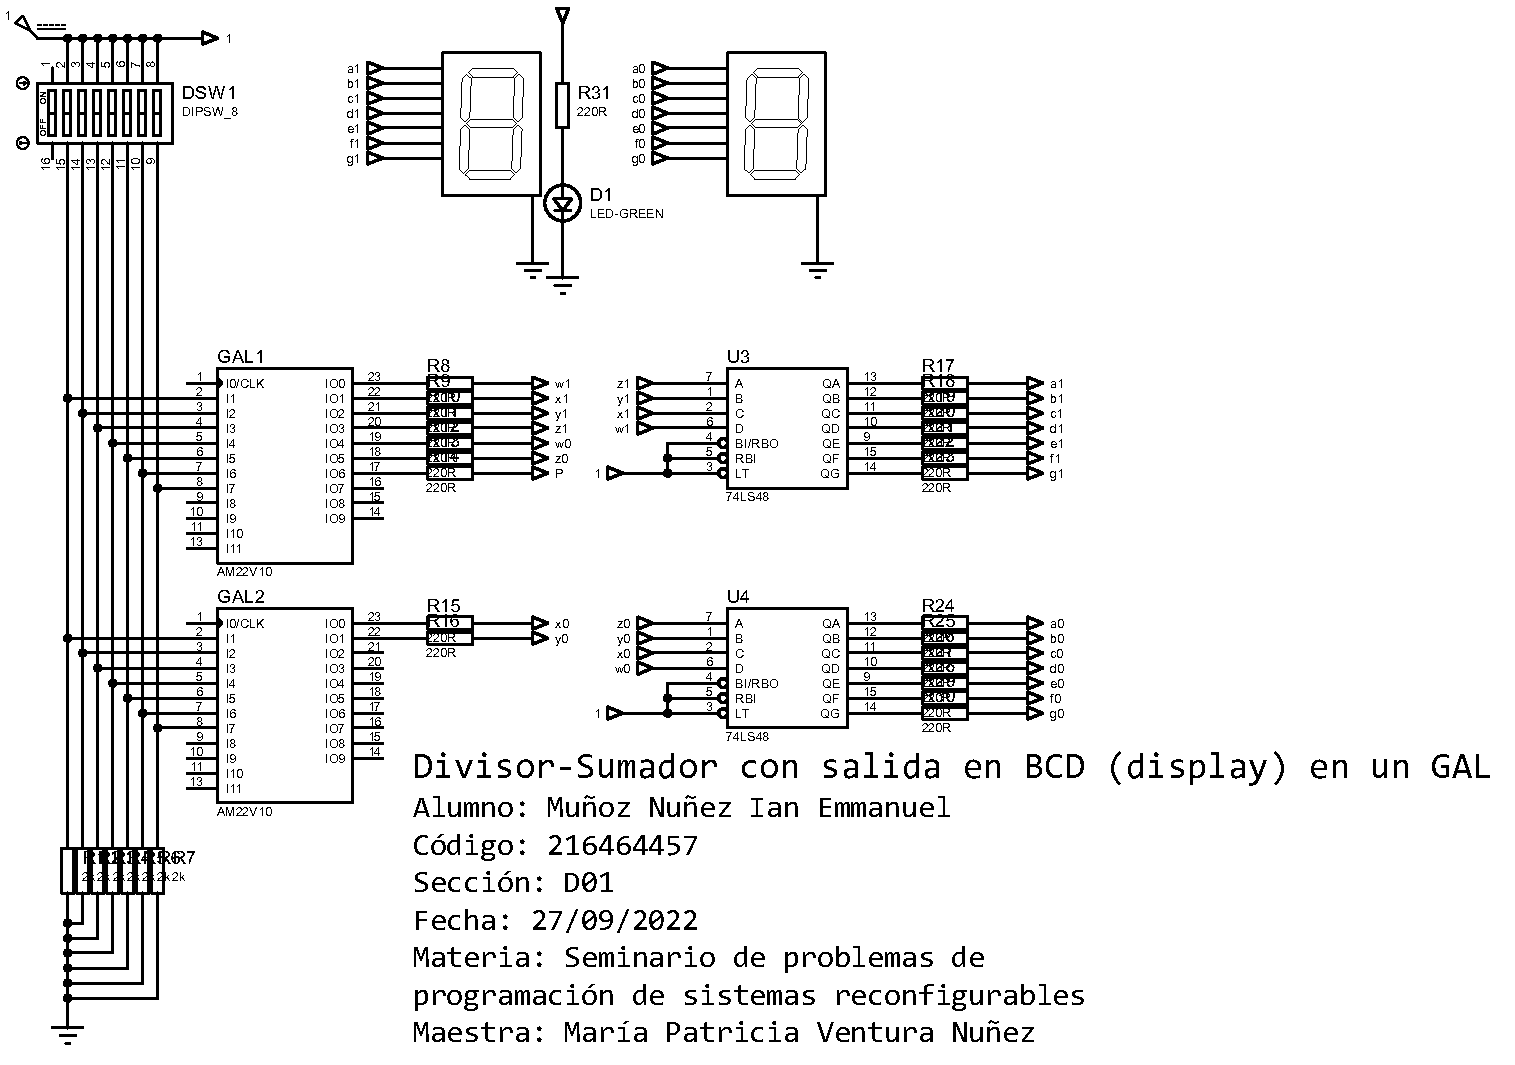
\includepdf[pages={1}]{main.PDF}
}

\subsection{Protoboard}
\begin{figure}[h!]
    \centering

    \begin{subfigure}{0.45\textwidth}
        \centering
        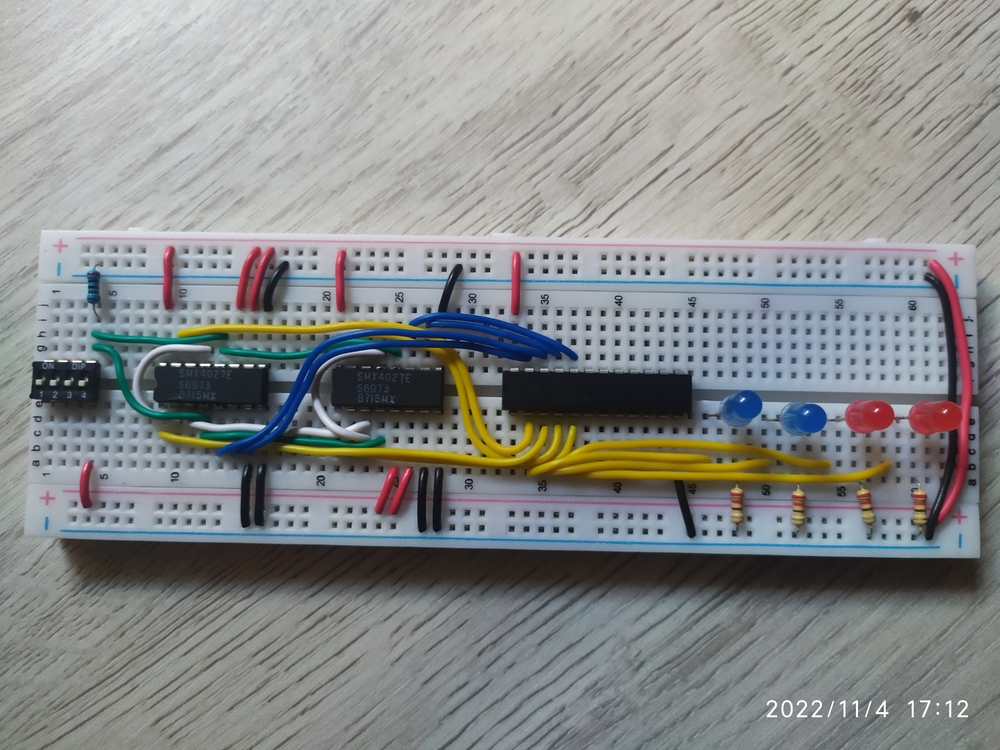
\includegraphics[width=\linewidth]{figs/IMG_20221104_171242.jpg}
    \end{subfigure}
    \begin{subfigure}{0.45\textwidth}
        \centering
        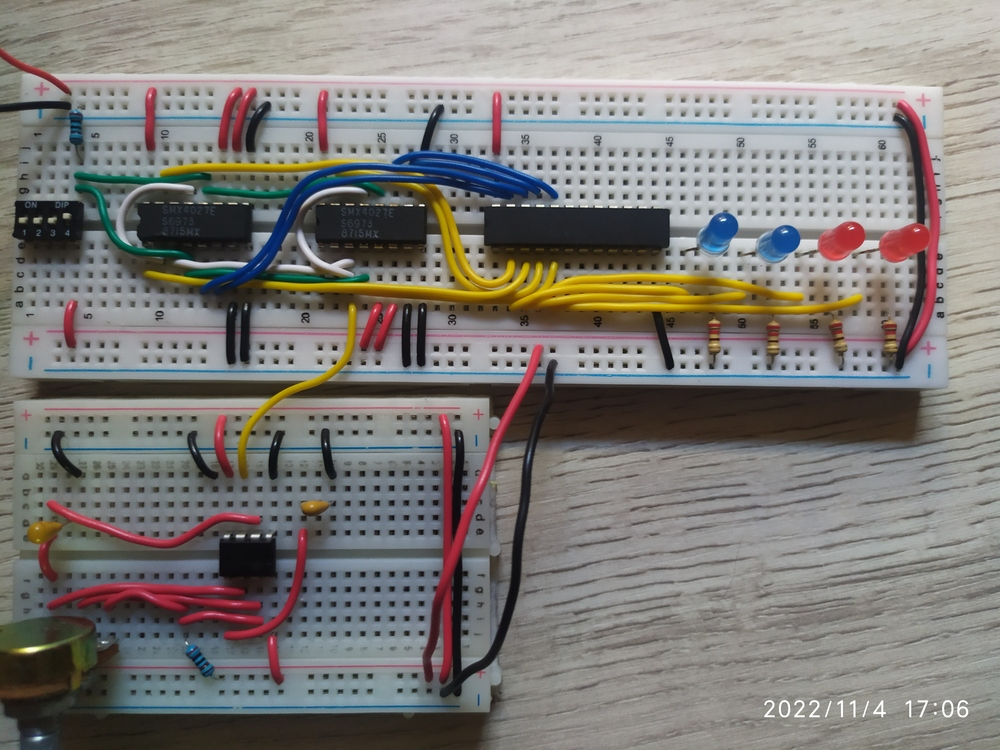
\includegraphics[width=\linewidth]{figs/IMG_20221104_170607.jpg}
    \end{subfigure}
    \begin{subfigure}{0.45\textwidth}
        \centering
        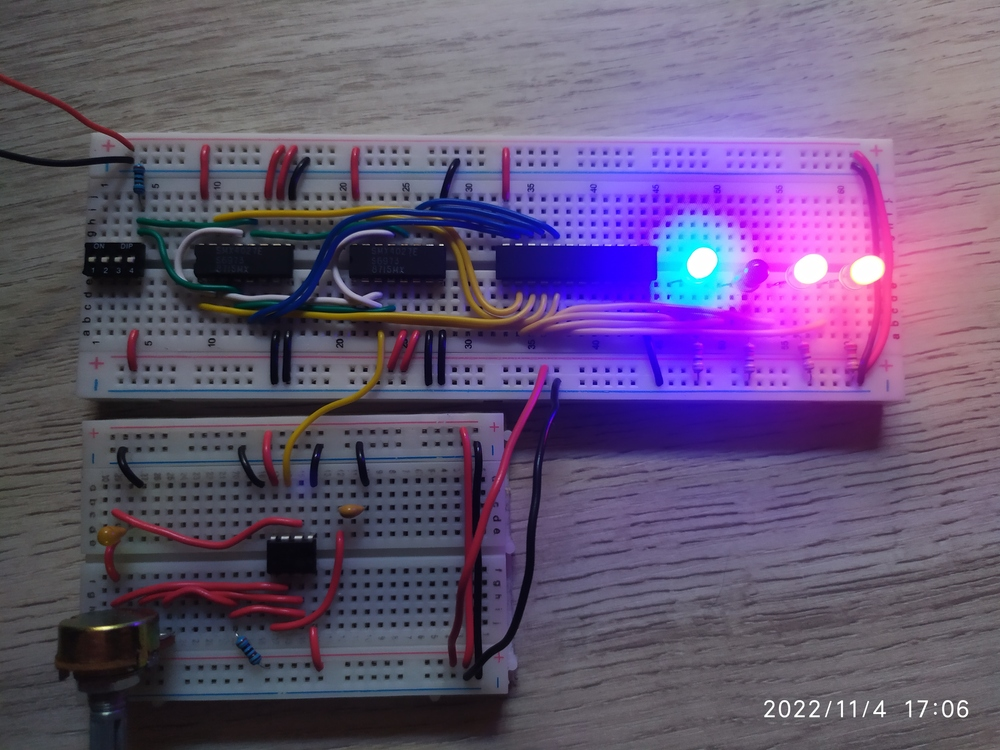
\includegraphics[width=\linewidth]{figs/IMG_20221104_170641.jpg}
    \end{subfigure}
    \begin{subfigure}{0.45\textwidth}
        \centering
        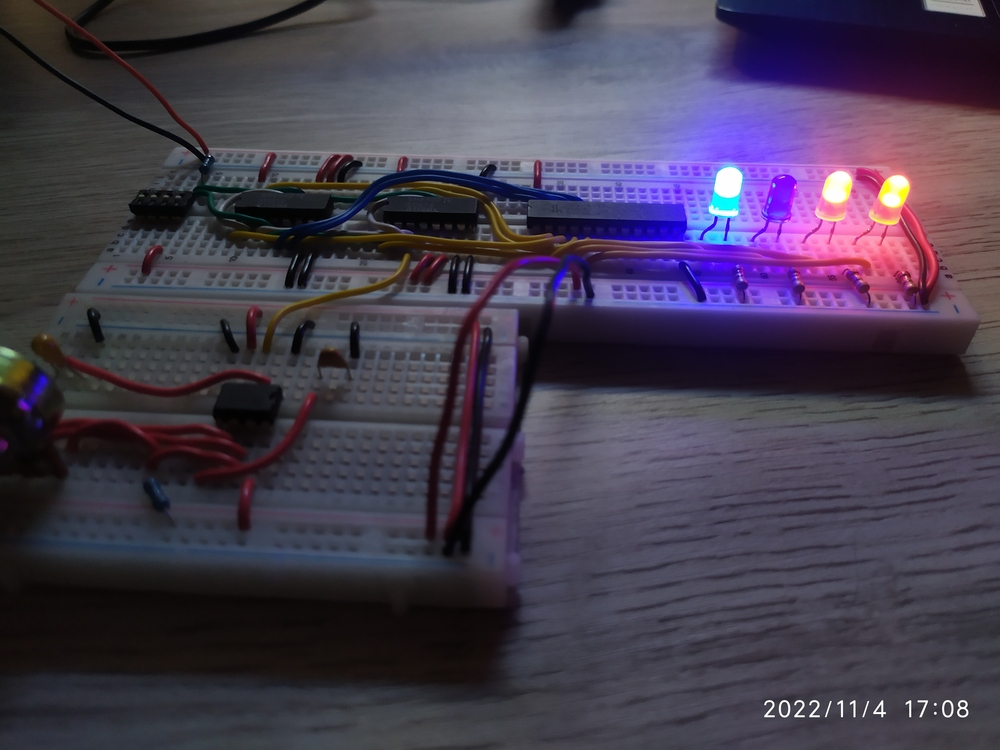
\includegraphics[width=\linewidth]{figs/IMG_20221104_170809.jpg}
    \end{subfigure}
    \begin{subfigure}{0.45\textwidth}
        \centering
        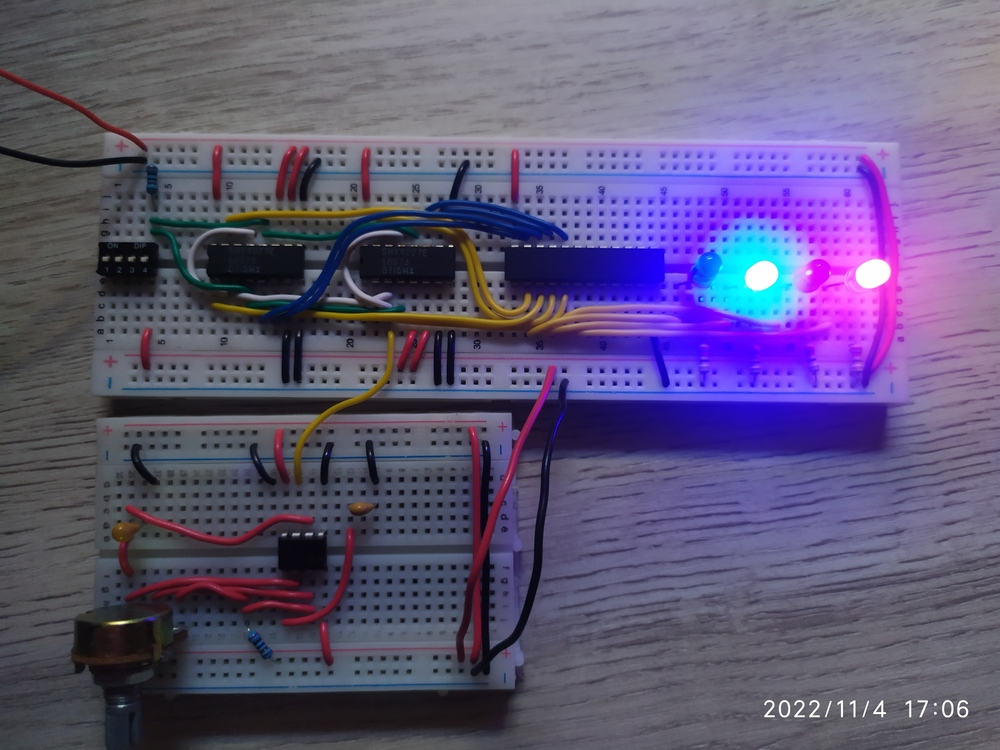
\includegraphics[width=\linewidth]{figs/IMG_20221104_170634.jpg}
    \end{subfigure}
    \begin{subfigure}{0.45\textwidth}
        \centering
        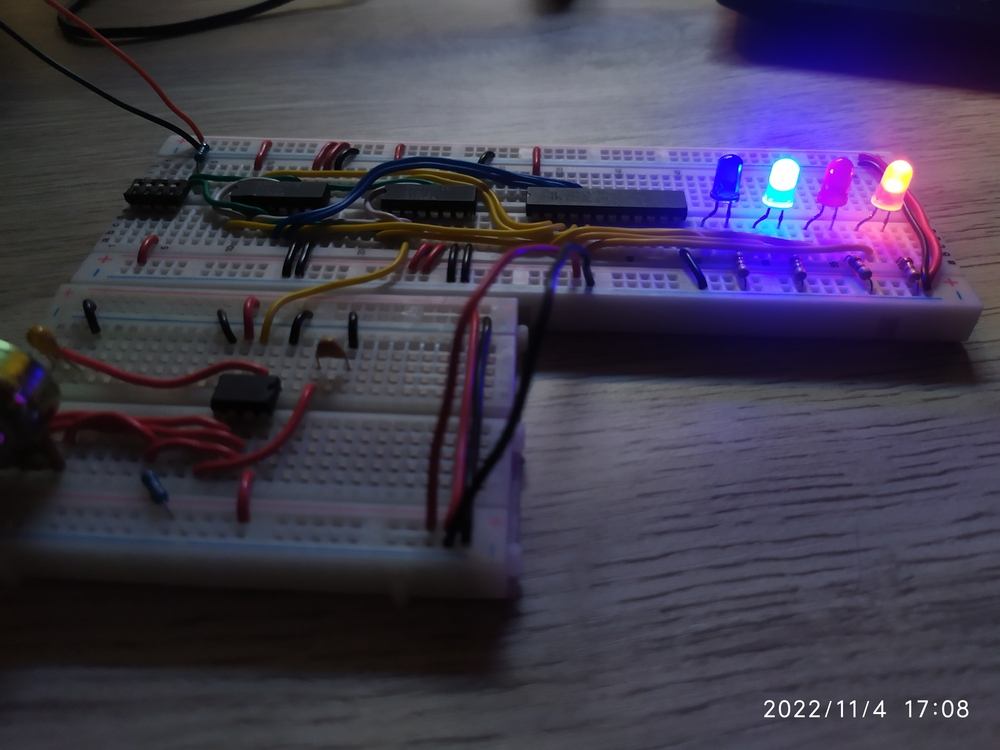
\includegraphics[width=\linewidth]{figs/IMG_20221104_170802.jpg}
    \end{subfigure}

    \caption{\sffamily Circuito en protoboard}
    \label{fig:proto}

\end{figure}

\section{Conclusión}
{\sffamily\large
    \hspace{0.5cm} Fue interesante aprender a controlar las \emph{Flip-Flop's} para
    usarlas como mejor nos parezca, al principio es difícil entender el funcionamiento
    y como es que se manejan las F-F's de manera asíncrona, pero al final el resultado
    es muy impresionante y reconfortante.

}

\end{document}

